% !TeX program = xelatex
% 接在 3.4 之後，沿用 amsmath、amssymb 與既有論文主檔。

% ==================================================
% 3.5 視覺目標估測與任務參考生成
% ==================================================
\section{視覺目標估測與任務參考生成}
\label{sec:visual_task_reference}

移動操作所需的參考包含物件位置、抓取方向、底盤接近位置及操作進度。Mittal 等人\cite{mittal2022articulated}將 RGB-D 感知、物件操作規劃與全身控制整合，呈現感知資訊與操作模型銜接的重要性。本研究結合 Mask R-CNN 實例分割與深度幾何估測更新操作目標，再依導航可達性與手臂構型產生控制參考。


% ==================================================
% 3.5.1 任務目標之視覺定位與幾何估測
% ==================================================
\subsection{任務目標之視覺定位與幾何估測}
\label{subsec:visual_geometric_estimation}

住宅整合任務以 Mask R-CNN\cite{he2017maskrcnn}分割門把、門扇、圓柱、抽屜把手、筆狀代理物及抽屜面板六類目標。網路採 ResNet-50-FPN v2，以 COCO 預訓練權重初始化，再由 Isaac Sim 渲染 RGB 影像與語意標註建立訓練資料；同類的不同連通區域分別建立實例標註。模型輸出類別、信心分數、外框及遮罩，線上推論不使用語意真值。模擬影像測試集的類別平均遮罩 IoU 約為 0.754，真實影像及跨場域表現尚未驗證。
% 來源：evaluation/house_seg.py、evaluation/seg_vision.py、
% evaluation/experiments/20261119_m8_house_d2_unified91_result.json。

% ==================================================
% 3.5.1 英文參考圖：Mask R-CNN 原理
% ==================================================
Mask R-CNN 的原始流程如\cref{fig:ref_mask_rcnn_framework}所示，對候選區域同時提供類別、外框與實例遮罩。此圖用於說明原方法概念；本研究採用前述 ResNet-50-FPN v2 實作，並將遮罩連結至深度幾何估測。

\begin{figure}[htbp]
    \centering
    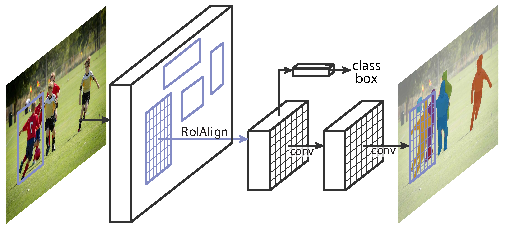
\includegraphics[width=0.95\textwidth]{figsrc/reference_figures/mask_rcnn_framework_he2017.pdf}
    \caption{Mask R-CNN 實例分割方法之原理示意（引自文獻\cite{he2017maskrcnn}之圖~1）}
    \label{fig:ref_mask_rcnn_framework}
\end{figure}

圓柱、筆、抽屜把手、面板及門扇以預測遮罩選取深度點，並依幾何估測需求進行遮罩內縮、有效距離及深度離群篩選。門把的幾何偵測需要保留門板平面與橫桿端部背景，因此以遮罩外框建立擴張 ROI 視窗，再於視窗內使用有效深度資料。遮罩決定待估測區域，物件半徑、高度、橫桿尺寸與機構軸向等已知資訊則提供幾何先驗。

令深度影像中像素座標為 $(u,v)$，其光軸深度為 $z(u,v)$，相機內參矩陣為 $K_C$。有效深度點在相機座標中的位置為
\begin{equation}
    {}^{C}p(u,v)
    =z(u,v)K_C^{-1}
      \begin{bmatrix}u&v&1\end{bmatrix}^{\top}.
    \label{eq:ch3_depth_backprojection}
\end{equation}
深度點經式\eqref{eq:ch3_visual_timestamp_transform}轉換至世界座標後，再依目標類型估計幾何。家具登錄資訊可提供任務導引與局部座標基準，住宅分割版本的深度點選取則由模型遮罩或門把 ROI 決定；較早以家具範圍進行幾何搜尋的版本另依其實際設定說明。

抽屜把手以面板點群估計櫃面方向，再由面板前方的橫桿點群取得桿心與高度。門扇開度則由鉸鏈附近的點群主方向估計，並核對可見長度及擬合直線與鉸鏈的距離。筆狀物件以點群主成分取得長軸方向，再利用長寬條件與頂面點估計中心。

對已知半徑 $r_o$ 的直立圓柱，令 $P_\ell^{xy}$ 為候選側面點的水平投影，以可見點群中心及半徑補償建立初值，再求解
\begin{equation}
    \hat c_o=
    \underset{c\in\mathbb R^2}{\operatorname{arg\,min}}
    \sum_{\ell}
    \left(\|P_\ell^{xy}-c\|-r_o\right)^2.
    \label{eq:ch3_known_radius_object_fit}
\end{equation}
式中以高斯牛頓法由初值迭代取得局部解。分割版本以可見點高度的高分位數估計頂面，再配合已知物件高度取得圓柱中心高度；繞對稱軸的方向由抓取需求選擇。筆狀物件的主軸具有 $\pi$ 方向歧義，需由可行抓取構型選擇對應方向。上述估測只輸出各物件可觀測且任務所需的幾何量，其餘分量由已知模型與操作條件決定。


本研究由分割至操作目標的資料流程如\cref{fig:ch3_mask_rcnn_target_pipeline}所示。遮罩與同一畫面的深度對應後，先建立相機座標中的幾何量，再以影像擷取時間對齊機器人狀態與相機外參，得到帶有來源時間的世界座標目標。門把分支保留擴張 ROI 所需的背景深度，各類目標依其幾何特性採用相應估測。

\begin{figure}[htbp]
    \centering
    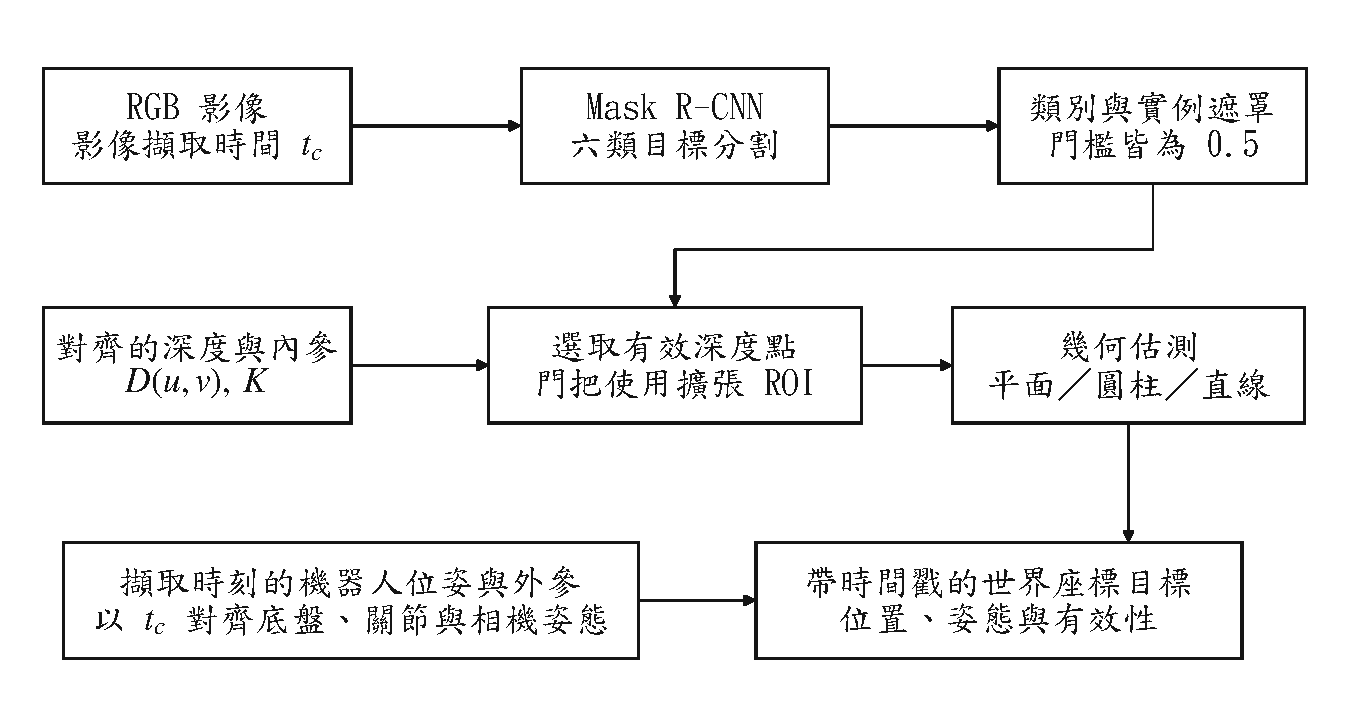
\includegraphics[width=0.98\textwidth]{figsrc/ch03/mask_rcnn_target_pipeline.pdf}
    \caption{本研究之實例分割、深度點選取與帶時間戳操作目標生成流程}
    \label{fig:ch3_mask_rcnn_target_pipeline}
\end{figure}

% ==================================================
% 3.5.2 影像、機器人狀態與座標轉換之時間對齊
% ==================================================
\subsection{影像、機器人狀態與座標轉換之時間對齊}
\label{subsec:visual_state_time_alignment}

機器人在影像取得與控制求解之間可能持續移動，因此，目標轉換須使用影像觀測時刻的相機位姿。令 $t_o$ 為觀測時間，世界座標中的量測點為
\begin{equation}
    \begin{bmatrix}{}^{W}p\\1\end{bmatrix}
    ={}^{W}T_C(t_o)
      \begin{bmatrix}{}^{C}p\\1\end{bmatrix},
    \qquad
    {}^{W}T_C(t_o)
    ={}^{W}T_B(t_o)\,{}^{B}T_C(q_a(t_o)).
    \label{eq:ch3_visual_timestamp_transform}
\end{equation}
對固定於底盤的相機，$ {}^{B}T_C$ 為固定外參；對手腕相機，則包含手臂運動鏈與相機安裝偏移。使用平台狀態與模型外參時，須保留其座標定義及來源時間。

目標封包保留觀測時間、座標系、估計幾何與有效性資訊。影像處理完成後仍沿用原觀測時間，並在接近或抓持前檢查資料新鮮度、可見點數與幾何一致性。對暫時遮蔽的目標，可在既定有效時間內保留估計；超過條件時重新觀測或停止該階段的推進。

底盤相機與手腕相機依可見性及任務階段提供觀測。當次實驗使用的來源、更新時機及保留策略分別記錄，避免將不同來源的結果視為同一時刻的量測。

% ==================================================
% 3.5.2 視覺量測與相機位姿依觀測時間配對之流程
% ==================================================
視覺量測與相機位姿的時間配對如\cref{fig:ch3_visual_time_alignment}所示。影像處理完成後仍保留原觀測時間 $t_o$，並使用該時刻的相機位姿進行座標轉換，再將世界座標中的目標提供給操作參考生成。

\begin{figure}[htbp]
    \centering
    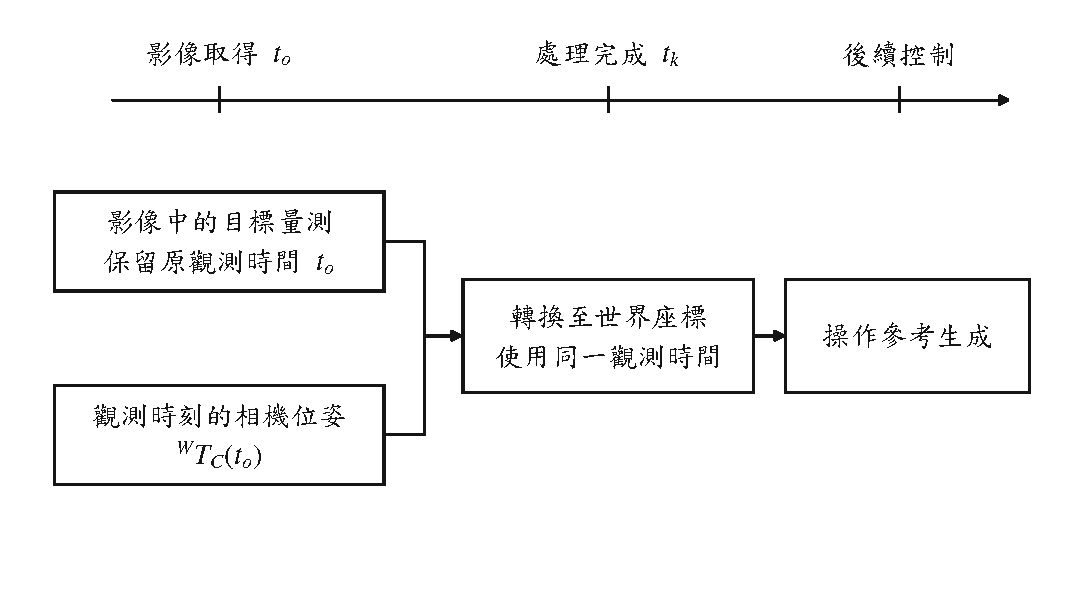
\includegraphics[width=0.98\textwidth]{figsrc/ch03/visual_time_alignment.pdf}
    \caption{視覺量測與相機位姿依觀測時間配對之流程}
    \label{fig:ch3_visual_time_alignment}
\end{figure}

% ==================================================
% 3.5.3 可行操作區域與底盤目標選擇
% ==================================================
\subsection{可行操作區域與底盤目標選擇}
\label{subsec:feasible_operation_base_selection}

操作目標確定後，需選擇可由導航到達、且手臂能完成接近與抓持的底盤位置。候選由目標與家具幾何生成，再檢查底盤淨空、最新未知障礙點、關節限制、預抓與抓取構型，以及相關路段的可達性。

以圓柱物件的候選評分為例，令 $\mathcal F_k$ 為本次通過檢查的有限候選集合，採用
\begin{equation}
    (b^{*},q_a^{*})
    =\underset{(b,q_a)\in\mathcal F_k}{\operatorname{arg\,min}}
      \left[
        w_L L_{\mathrm{route}}(b)
        +\frac{w_\sigma}
         {\max(\sigma_{\min}(J_{\mathrm{sel}}(q_a)),\epsilon_\sigma)}
        +w_{\mathrm{ext}}\ell_{\mathrm{ext}}^2(b,q_a)
      \right],
    \label{eq:ch3_operation_base_selection}
\end{equation}
其中 $b=[x_B,y_B,\theta_B]^{\top}$，$L_{\mathrm{route}}$ 為路線長度估計，$J_{\mathrm{sel}}$ 為選位評估使用的手臂雅可比，$\epsilon_\sigma>0$ 用於避免分母接近零。$\ell_{\mathrm{ext}}$ 定義為手臂基座至 TCP 的水平伸展距離：
\begin{equation}
    \ell_{\mathrm{ext}}(b,q_a)
    =\left\|\Pi_{xy}\left({}^{W}p_E(b,q_a)-{}^{W}p_A(b)\right)\right\|_2,
    \qquad
    \Pi_{xy}=\begin{bmatrix}1&0&0\\0&1&0\end{bmatrix}.
    \label{eq:ch3_operation_extension_cost}
\end{equation}
此項用於在可行候選中降低過度伸展的偏好；權重為非負值，依實驗設定揭露。既有選位程式及已完成對照批次對應 $w_{\mathrm{ext}}=0$；正權重伸展項為本次新增設計，尚待實作與 Isaac 驗證，不回溯套用於既有結果。
% 狀態：evaluation/cyl_reach_map.py 的 select() 目前只有路線與奇異值項。
% 新伸展項需接入程式、保存配置並完成 Isaac 驗證後，才改述為已啟用。

啟用格點路線評估時，由已知家具及未知回波建立可行域，並以 Dijkstra 最短路徑方法\cite{dijkstra1959note}取得路線成本。不同任務可依後續目標及朝向增加評分項。

選定候選提供導航目標、操作朝向與可用構型，實際接近路徑仍由導航前端更新。候選區域與路線需配合新觀測重新核對；式\eqref{eq:ch3_operation_base_selection}的選擇範圍為當次已生成且已檢查的候選集合。

底盤選位前後的操作關係如\cref{fig:ch3_visual_operation_reference}所示。系統依已定位目標與家具幾何產生底盤候選，通過淨空、路線與手臂構型檢查後，再依評分選擇操作位姿。選定結果提供導航接近目標與可用手臂構型，後續仍依實際狀態更新控制參考。

\begin{figure}[htbp]
    \centering
    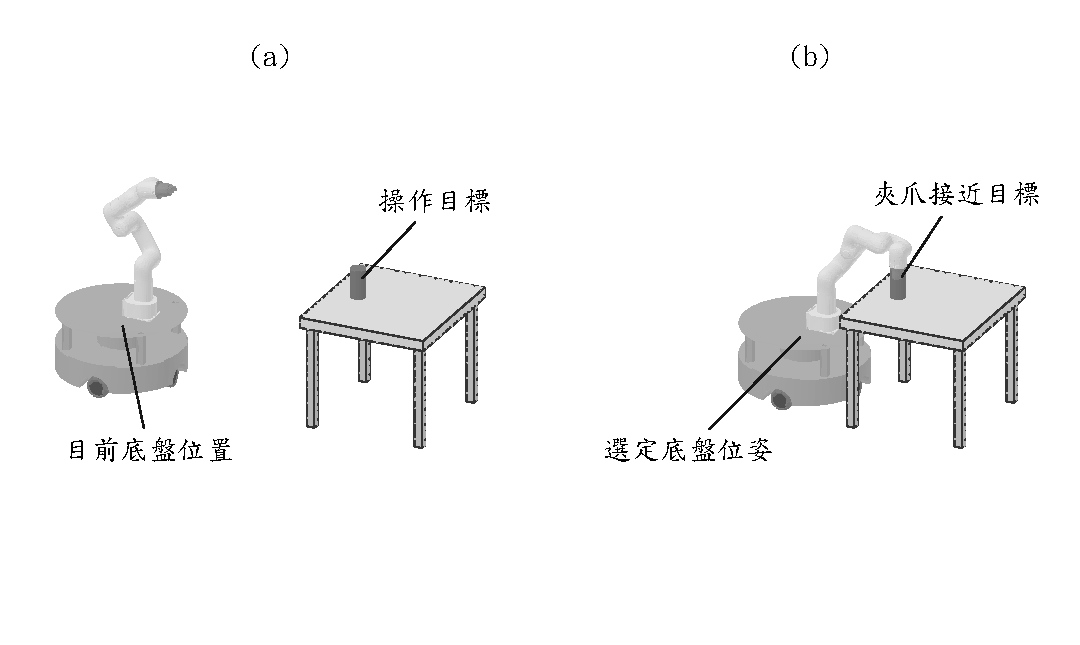
\includegraphics[width=0.98\textwidth]{figsrc/ch03/visual_operation_reference.pdf}
    \caption{操作目標導引之底盤選位：(a) 選位前的機器人與目標位置；(b) 選位後，手臂接近目標。}
    \label{fig:ch3_visual_operation_reference}
\end{figure}

% ==================================================
% 3.5.4 導航路徑下之朝向與末端參考生成
% ==================================================
\subsection{導航路徑下之朝向與末端參考生成}
\label{subsec:navigation_manipulation_reference}

圓柱接近階段採用關節空間展開與後段併線；第 101 趟 Isaac 紀錄已出現對應分支事件並完成圓柱抓取、抬升與放盒。該趟回程因門扇視覺估測錯誤而停止，故此處僅確認圓柱階段的執行，不視為整趟任務通過。移動中接近時，底盤沿導航路徑行進，操作端依剩餘距離調整朝向、手臂展開進度及抓取線的推進。對已啟用此改版的圓柱接近階段，先指定中間關節構型，再由全身正向運動學建立末端參考；其他任務仍依各自啟用的參考策略處理。

令 $\theta_{\mathrm{nav},i}$ 為導航朝向，$\theta_g$ 為操作朝向，以距離權重 $w_i\in[0,1]$ 建立
\begin{equation}
    \theta_{r,i}=\theta_{\mathrm{nav},i}
    +w_i\operatorname{wrap}(\theta_g-\theta_{\mathrm{nav},i}),
    \label{eq:ch3_operation_heading_reference}
\end{equation}
其中 $\operatorname{wrap}(\cdot)$ 將角度差映射至 $(-\pi,\pi]$。接近時逐步增加 $w_i$，離開抓取階段後再依任務條件交回導航朝向。

採用五次端點平滑函數 $\psi(\nu)=10\nu^3-15\nu^4+6\nu^5$\cite{flash1985coordination}。令 $d_i$ 為預測底盤至操作位置的距離，定義距離進度並限制其增加速度：
\begin{equation}
    \begin{aligned}
        \nu_i^{\mathrm{dist}}
        &=\operatorname{clip}\!\left(
          \frac{d_{\mathrm{out}}-d_i}{d_{\mathrm{out}}-d_{\mathrm{in}}},0,1\right),\\
        \nu_i&=\min\!\left(\nu_i^{\mathrm{dist}},
          \nu_k+\frac{t_i-t_k}{T_{\mathrm{exp,min}}}\right),
        \qquad \beta_i=\psi(\nu_i).
    \end{aligned}
    \label{eq:ch3_distance_based_arm_progress}
\end{equation}
其中 $\nu_k$ 為目前已承接的展開進度，$T_{\mathrm{exp,min}}>0$ 為最短展開時間參數；實作以基準最短時間及最大關節位移所需時間之較大者設定，關節速度目標另由控制限制處理。進度由距離與狀態更新，五次函數用於平滑端點，不將整段運動等同於固定時間的最小急動軌跡。

令 $q_{a,0}$ 為展開開始時的實際關節構型，$q_a^g$ 為選位所得的抓取構型，關節展開參考為
\begin{equation}
    q_{a,i}^{\mathrm{exp}}
      =q_{a,0}+\beta_i(q_a^g-q_{a,0}),
    \qquad
    T_{E,i}^{\mathrm{exp}}
      =\operatorname{FK}_{\mathrm{WB}}(\widehat b_i,q_{a,i}^{\mathrm{exp}}),
    \label{eq:ch3_joint_space_unfold_reference}
\end{equation}
其中 $\widehat b_i$ 為相應預測時刻的底盤位姿。由此建立的末端參考保留展開構型與底盤運動的對應關係；關節構型參考亦可作為同一全身控制問題的姿態引導，與末端目標共同使用。展開路徑仍需核對關節限制、環境及自身淨空。

後段再銜接世界座標中的預抓或抓取線。令 $\beta_0\in[0,1)$ 為開始併線的進度，定義
\begin{equation}
    \gamma_i=\psi\!\left(\operatorname{clip}
        \left(\frac{\beta_i-\beta_0}{1-\beta_0},0,1\right)\right).
    \label{eq:ch3_late_merge_weight}
\end{equation}
將 $T_{E,i}^{\mathrm{exp}}$ 的位置與姿態記為 $(p_{\mathrm{exp},i},R_{\mathrm{exp},i})$，抓取線目標記為 $(p_{\mathrm{line},i},R_{\mathrm{line},i})$，則最終末端參考為
\begin{equation}
    \begin{aligned}
        p_{E,i}^{d}
        &=(1-\gamma_i)p_{\mathrm{exp},i}+\gamma_i p_{\mathrm{line},i},\\
        R_{E,i}^{d}
        &=R_{\mathrm{exp},i}\exp\!\left(
          \gamma_i\log(R_{\mathrm{exp},i}^{\top}R_{\mathrm{line},i})\right).
    \end{aligned}
    \label{eq:ch3_continuous_approach_reference}
\end{equation}
前段依關節構型展開，後段隨 $\gamma_i$ 增加而併入抓取線；$\beta_i=1$ 時直接採用抓取線目標。抓取線推進仍由底盤位置及 TCP 到位狀態觸發，閉爪依抓持條件判定。朝向或位置參考變更後，依式\eqref{eq:ch3_reference_velocity_reconstruction}重新計算底盤參考速度，再建立末端追蹤與命令限制。


% ==================================================
% 3.5.4 距離限速與手臂展開進度示意
% ==================================================
\cref{fig:ch3_mobile_approach_distance_profile}以第 101 趟圓柱參考封包的參數說明距離剖面。逐軸平移速度上限在剩餘距離 $1.3$ 至 $0.4$ m 間，以三次平滑函數由 $0.26$ 降至 $0.06$ m/s；距離展開進度則在 $1.2$ 至 $0.3$ m 間由零增加至一，超過 $\beta_0=0.55$ 後逐步併入抓取線。圖中顯示距離規則的設計曲線，實際進度另受最短展開時間限制，最終速度由導航、障礙、家具鄰近條件及輪級限制共同決定。閉爪與確認仍依實測到位及抓持條件觸發。

\begin{figure}[htbp]
    \centering
    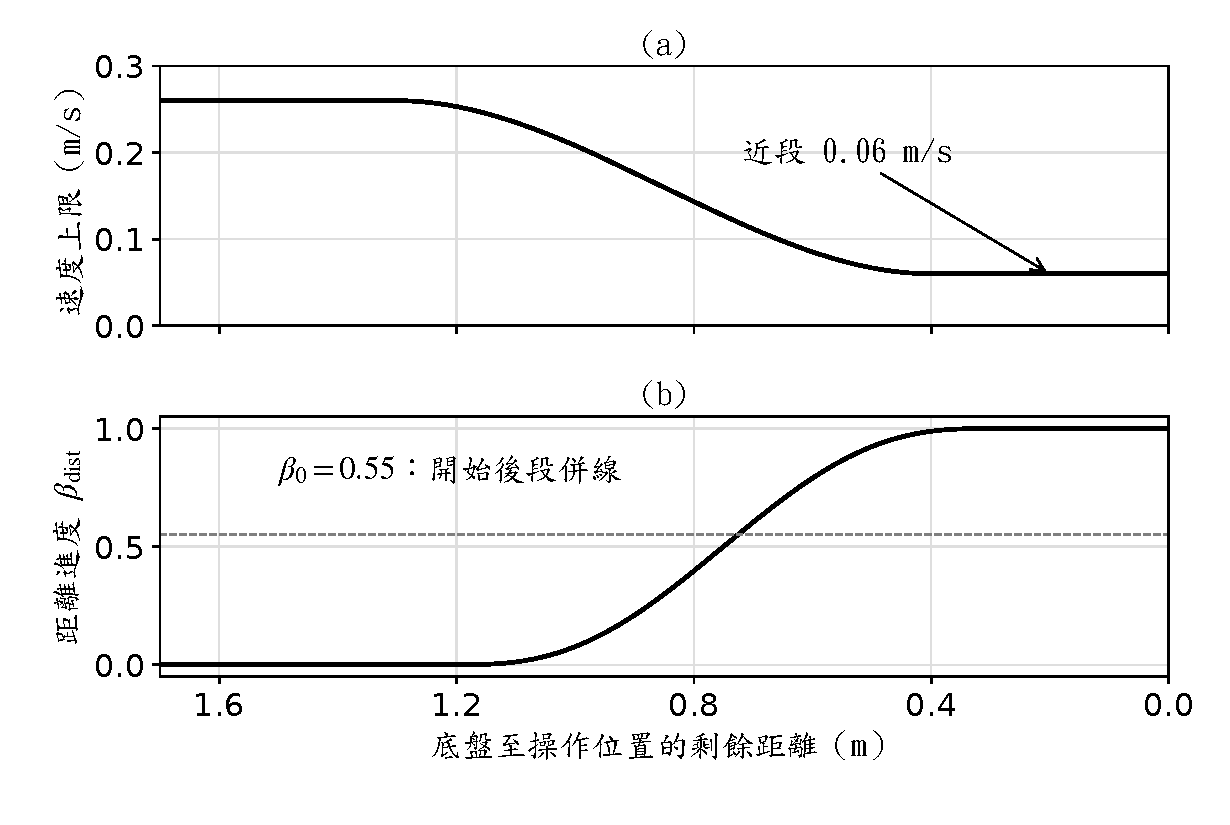
\includegraphics[width=0.94\textwidth]{figsrc/ch03/mobile_approach_distance_profile.pdf}
    \caption{圓柱接近階段之距離規則：(a) 平移逐軸速度上限；(b) 手臂距離展開進度與後段併線門檻。圖中為設計曲線，實際進度另受時間與狀態限制。}
    \label{fig:ch3_mobile_approach_distance_profile}
\end{figure}
% 證據：evaluation/runs/m8house_d2_unified_101/world.log，
% pick_jblend_start t=90.06、CLOSE t=105.46（位置誤差 1.27 mm）、BIN_MOVE t=107.96。
% 此圖不是量測速度曲線，亦未由真實軌跡重建未記錄的 beta。
